\documentclass{beamer}
\usetheme{Madrid}
\usepackage[utf8]{inputenc}
\usepackage[portuguese]{babel}
\usepackage[T1]{fontenc}
\usepackage{amsmath}
\usepackage{amsfonts}
\usepackage{amssymb}
\usepackage{tikz}
\usepackage{pdfpages}
\usepackage{graphicx}
\author{Dingchao Gao}
\title{Quantum Circuit Transformation For Neutral atom computation}
% \subtitle{QCT for NA}
\setbeamercovered{transparent} 
%\setbeamertemplate{navigation symbols}{} 
%\logo{\includegraphics[scale=.7]{LogoCentralDataShow}} 
\institute{ISCAS} 
\date{\today} 
%\subject{} 
\usepackage{xcolor}
\usepackage{bm}
\definecolor{darkorange}{rgb}{1.0, 0.55, 0.0} 

\tikzset{
    DasAtomStyle/.style={color=black, ultra thick},
    TetrisStyle/.style={color=darkorange,ultra thick, dashed},
    EnolaStyle/.style={color=green!50!black,ultra thick, dotted},
    AtomiqueStyle/.style={color=red!70!black, ultra thick, loosely dash dot}
}
\usetikzlibrary{calc,patterns}
\usetikzlibrary{shapes.geometric, arrows, positioning}
\usepackage{pgfplots}
\pgfplotsset{compat=1.18}
\pgfplotsset{max space between ticks=50pt}
\usepackage{yquant}
 \usepackage{booktabs} 
\AtBeginSection[]
{
\begin{frame}{contents}
\transfade
\tableofcontents[sectionstyle=show/shaded,subsectionstyle=show/shaded/hide]
\addtocounter{framenumber}{-1} 
\end{frame}
}

\begin{document}
% Title page

\begin{frame}
    \titlepage
\end{frame}
\begin{frame}{Main reference}
    \begin{itemize}
        \item \href{https://arxiv.org/abs/2409.03185}{DasAtom: A Divide-and-Shuttle Atom Approach to Quantum Circuit Transformation,Yunqi Huang and Dingchao Gao and Shenggang Ying and Sanjiang Li}
        \item \href{https://arxiv.org/abs/2309.08656}{Computational Capabilities and Compiler Development for Neutral Atom Quantum Processors: Connecting Tool Developers and Hardware Experts}
        
    \end{itemize}
\end{frame}
\section{background}
\subsection{motivation}
\begin{frame}
    \frametitle{sparse qubit connectivity}
    \begin{itemize}
        \item controlled operations
        \item NISQ architectures:
        \begin{figure}
            \centering
            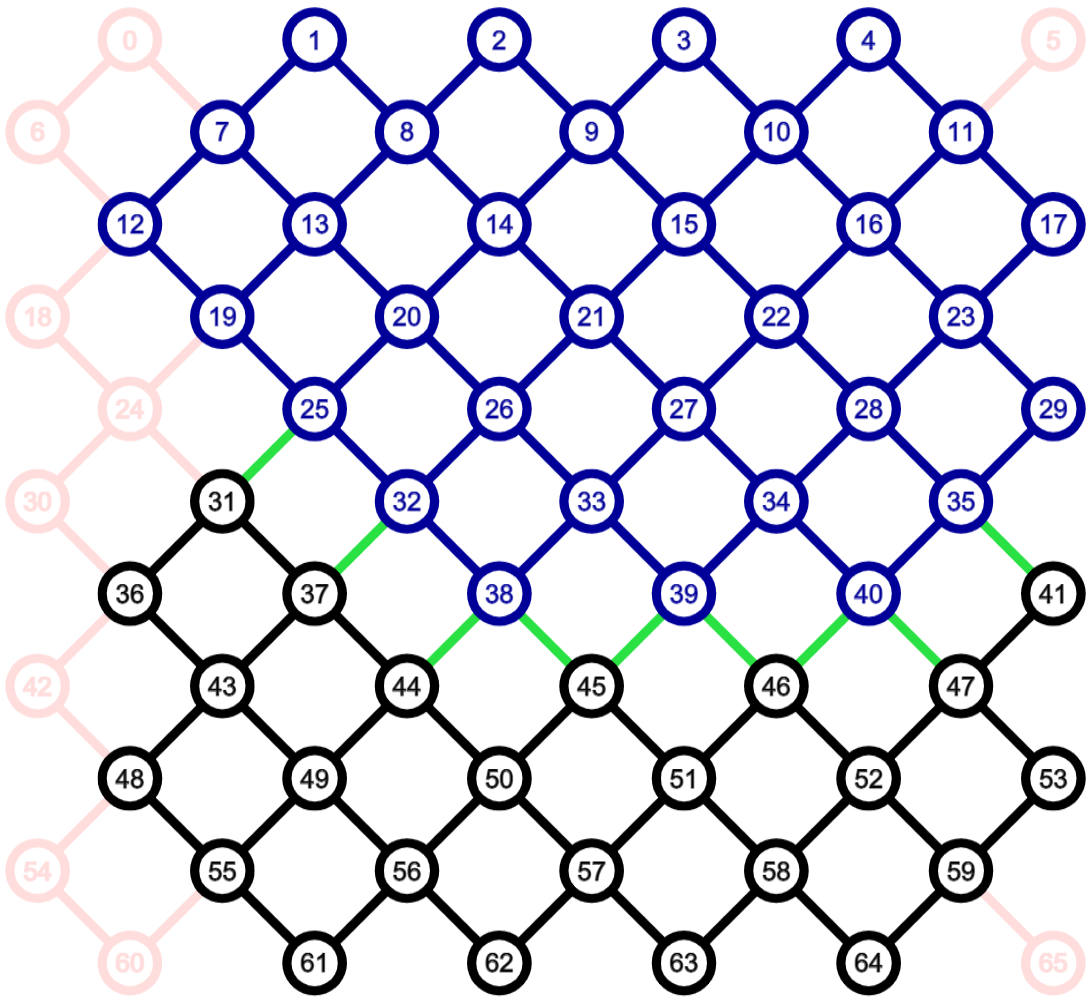
\includegraphics[width=.3\linewidth]{figure/connection.png}
            \caption{Qubit ordering and optimal cut for 56-qubit circuit
            with 20 cycles in \cite{Nash_2020}}
        \end{figure} 
    \end{itemize}
\end{frame}
\begin{frame}
    \frametitle{different sequence of operations}
    \begin{columns}
        \column{0.5\textwidth}
        \begin{minipage}[c][0.4\textheight][c]{\linewidth}
            \centering
            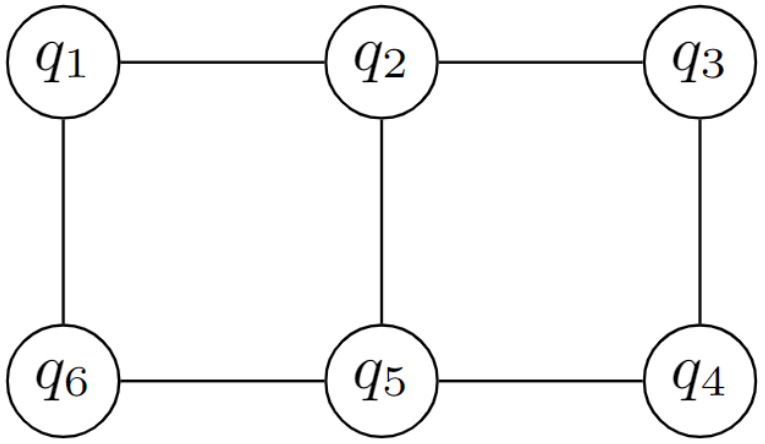
\includegraphics[width=0.8\linewidth]{figure/example.png}
        \end{minipage}
        
        \column{0.5\textwidth} % remember add this to the other clumn
        \begin{minipage}[c][0.4\textheight][c]{\linewidth}
            \centering
            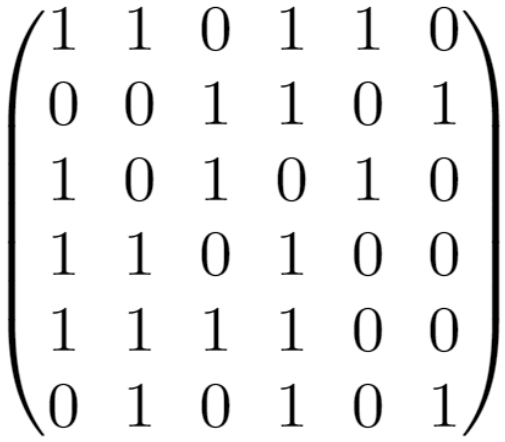
\includegraphics[width=0.8\linewidth]{figure/linear.png}
        \end{minipage}
    \end{columns}
\end{frame}
\subsection{result}
\begin{frame}
    \frametitle{linear reversible circuit synthesis}
    \begin{itemize}
        \item input: the qubit connectivity graph and a binary matrix
        \item $O\left(\frac{n^{3}}{\log {n}} \right)$ VS $O\left(n^{2}\right)$
        \item universal set
        % TODO: need figure 8
    \end{itemize}
\end{frame}
\section{Related Work}

\subsection{Compilation Frameworks for Neutral Atom Quantum Computing}

\begin{frame}{Compilation Steps in NAQC}
    \frametitle{Compilation Process in Neutral Atom Quantum Computing}
    \begin{itemize}
        \item \textbf{Platform-independent Compilation}
            \begin{itemize}
                \item Applies general optimizations (e.g., loop unrolling, gate commutation)
            \end{itemize}
        \item \textbf{Platform-dependent Compilation}
            \begin{itemize}
                \item Adapts quantum circuits to specific hardware constraints and capabilities
            \end{itemize}
        \item \textbf{Hardware-dependent Compilation}
            \begin{itemize}
                \item Translates abstract operations into hardware-executable instructions
            \end{itemize}
    \end{itemize}
\end{frame}

\begin{frame}
    \frametitle{Primary Goals of Platform-dependent Compilation}
    \begin{itemize}
        \item \textbf{Synthesis}
            \begin{itemize}
                \item Decompose complex gates into native hardware-compatible operations
            \end{itemize}
        \item \textbf{Mapping}
            \begin{itemize}
                \item Assign logical qubits to physical qubits, introducing SWAP or MOVE operations as needed
            \end{itemize}
        \item \textbf{Scheduling}
            \begin{itemize}
                \item Optimize gate execution timing to maximize parallelism and minimize errors
            \end{itemize}
    \end{itemize}
    \vspace{0.5em}
    \textbf{Considerations:}
    \begin{itemize}
        \item NAQC-specific features like atom shuttling and Rydberg interactions influence all compilation steps
        \item Compilation steps are often optimized collectively to accommodate hardware constraints
    \end{itemize}
\end{frame}

\begin{frame}{Challenges in NAQC Compilation}
    \frametitle{Compilation Challenges for Neutral Atom Quantum Computing}
    \begin{itemize}
        \item \textbf{Synthesis}
            \begin{itemize}
                \item Superconducting (SC) platforms support only one- and two-qubit gates, complicating multi-qubit operations in NAQC
            \end{itemize}
        \item \textbf{Mapping}
            \begin{itemize}
                \item SC relies on virtual swaps for qubit connectivity
                \item NAQC utilizes interaction radius (\( r_{\text{int}} \)) to define qubit coupling
            \end{itemize}
        \item \textbf{Scheduling}
            \begin{itemize}
                \item NAQC constraints from interaction radius require tailored scheduling strategies
            \end{itemize}
    \end{itemize}
\end{frame}

\subsection{Existing Compilation Approaches}

\begin{frame}{Compilation Strategies in NAQC}
    \frametitle{Overview of Compilation Strategies}
    \begin{itemize}
        \item NAQC introduces unique challenges and capabilities
        \item Existing works address these through various approaches:
            \begin{itemize}
                \item \textbf{Long-range Interaction Management}
                \item \textbf{Multi-qubit Gate Optimization}
                \item \textbf{Atom Shuttling Operations}
                % \item \textbf{Adaptation of SC Compilers}
            \end{itemize}
    \end{itemize}
\end{frame}

\begin{frame}{Long-range Interaction Compilers}
    \frametitle{Long-range Interaction Compilation Approaches}
    \href{https://arxiv.org/pdf/2111.06469}{Baker et al.\tiny{Exploiting Long-Distance Interactionsand Tolerating Atom Loss in Neutral Atom Quantum Architectures}}
    \begin{itemize}
        \item \textbf{Focus:} Qubit mapping and atom loss mitigation
        \item \textbf{Features:}
            \begin{itemize}
                \item Parallel SWAP execution
                \item Look-ahead optimization schemes
            \end{itemize}
    \end{itemize}
    
    \vspace{0.5em}
    \href{https://ieeexplore.ieee.org/abstract/document/10082942/}{Q-Tetris \tiny{Timing-Aware Qubit Mapping and Gate Scheduling Adapted to Neutral Atom Quantum Computing}}
    \begin{itemize}
        \item \textbf{Approach:} Greedy heuristic algorithm combined with Monte Carlo tree search
        \item \textbf{Advantages:}
            \begin{itemize}
                \item Time-efficient optimization
            \end{itemize}
    \end{itemize}
\end{frame}

\begin{frame}{Multi-qubit Gate Compilation}
    % \frametitle{Geyser: Multi-qubit Compilation Approach}
    % \textbf{Geyser \cite{Geyser29, Geyser115}}
    \href{https://dl.acm.org/doi/10.1145/3470496.3527428}{Geyser: a compilation framework for quantum computing with neutral atoms}
    \begin{itemize}
        \item \textbf{Approach:} Novel method for multi-qubit operations
        \item \textbf{Key Features:}
            \begin{itemize}
                \item Decomposes Toffoli gates into two-qubit gates
                \item Utilizes Qiskit for qubit mapping
                \item Optimizes laser pulse count
            \end{itemize}
        % \item \textbf{Evaluation Metrics:}
        %     \begin{itemize}
        %         \item Comparison of laser pulse count versus gate count
        %     \end{itemize}
    \end{itemize}
\end{frame}

\begin{frame}{Shuttling-based Compilation Approaches}
    \textbf{DPQA}
    \begin{itemize}
        \item \textbf{SMT based:}\href{http://arxiv.org/abs/2401.13807}{OLSQ-DPQA}
        \begin{itemize}
            \item \href{http://arxiv.org/abs/2405.15095}{Enola}
            \item \href{http://arxiv.org/abs/2311.15123}{Atomique}
            \item \href{https://arxiv.org/abs/2311.16190}{Q-pilot}
        \end{itemize}
    \end{itemize}
% \end{frame}

% \begin{frame}{Shuttling-based Compilation Approaches (2/2)}
%     \frametitle{Shuttling Compilation: Advanced Schemes}
    % \textbf{Schmid et al.}
    \href{http://arxiv.org/abs/2311.14164}{Schmid et al. \tiny{Hybrid Circuit Mapping: Leveraging the Full Spectrum of Computational Capabilities of Neutral Atom Quantum }}
    \begin{itemize}
        \item \textbf{Approach:} Hybrid compilation scheme
        \item \textbf{Features:}
            \begin{itemize}
                \item Employs SABRE-based heuristic
                \item Comprehensive support for various NAQC capabilities
            \end{itemize}
    \end{itemize}
\end{frame}

\subsection{Future Directions and Challenges}
% \begin{frame}{Comparison of Compilation Approaches}
%     \frametitle{Comparative Analysis of NAQC Compilation Strategies}
%     \tiny
%     \begin{tabular}{|l|l|l|l|}
%         \hline
%         \textbf{Approach} & \textbf{Focus} & \textbf{Key Features} & \textbf{Limitations} \\
%         \hline
%         Baker et al.& Qubit Mapping & Parallel SWAPs, Look-ahead & Limited to 1D \\
%         \hline
%         Q-Tetris & Optimization & Greedy Heuristics,MCTS & May miss global optima \\
%         \hline
%         Geyser& Multi-qubit Gates & Toffoli decomposition, Qiskit & Complexity increases with gates \\
%         \hline
%         Tan et al. & DPQA & 2D Shuttling & May require specific hardware \\
%         \hline
%         Schmid et al.& Hybrid & SABRE Heuristic, Comprehensive & Potentially higher computational cost \\
%         \hline
%     \end{tabular}
% \end{frame}
\begin{frame}{Future Challenges in NAQC Compilation}
    \frametitle{Future Challenges and Research Directions}
    \begin{itemize}
        \item \textbf{Synthesis Improvements}
            \begin{itemize}
                \item Enhance support for general quantum algorithms
                \item Integrate multi-qubit gate operations more effectively
            \end{itemize}
        \item \textbf{Capability Integration}
            \begin{itemize}
                \item Combine multiple NAQC-specific features seamlessly
            \end{itemize}
        \item \textbf{Error Analysis}
            \begin{itemize}
                \item Develop hardware-dependent error models
                \item Implement robust error mitigation techniques
            \end{itemize}
        \item \textbf{Platform Accessibility}
            \begin{itemize}
                \item Improve compiler usability and integration with diverse NAQC platforms
            \end{itemize}
    \end{itemize}
    \vspace{0.5em}
    \centering
    \textbf{Goal: Fully leverage the potential of the NAQC platform}
\end{frame}


\section{Our Work}

\subsection{DasAtom Framework}

\begin{frame}{Overview of DasAtom}
    \begin{itemize}
        \item \textbf{DasAtom} is a transformation framework for mapping quantum circuits onto neutral atom (NA) architectures.
        \item Leverages subgraph isomorphism to find optimal qubit mappings.
        \item Aims to enhance fidelity and efficiency by ensuring gates are directly executable.
    \end{itemize}
\end{frame}

\begin{frame}{Subgraph Isomorphism in Quantum Circuit Mapping}
    \begin{itemize}
        \item Uses subgraph isomorphism to map interaction graphs onto the NA grid.
        \item Ensures each gate in a subcircuit is directly executable.
        \item Embedding interaction graphs onto the NA grid enhances fidelity and efficiency.
    \end{itemize}

    % Optional illustrative figure
    % \begin{figure}
    % \centering
    % \includegraphics[width=0.8\linewidth]{interaction_graph_example.png}
    % \caption{Mapping the interaction graph onto the NA architecture using subgraph isomorphism.}
    % \end{figure}
\end{frame}
\begin{frame}{Running Example - Partition}
\begin{figure}
    \centering
\scalebox{0.7}{
\begin{tikzpicture}
\begin{scope}[scale=0.8]
    \begin{yquant}
    qubit {\Large $\reg_{\idx}$} q[5];
    zz (q[3], q[4]); barrier (q);
    zz (q[3], q[4]); barrier (q);
    zz (q[2], q[4]); barrier (q);
    zz (q[2], q[4]); barrier (q);
    zz (q[2], q[3]); zz (q[1], q[4]);
    barrier (q);
    zz (q[2], q[3]); zz (q[1], q[4]);
    barrier (q);
    zz (q[1], q[3]); zz (q[0], q[4]);
    barrier (q);
    zz (q[1], q[3]); zz (q[0], q[4]);
    barrier (q);
    zz (q[1], q[2]); zz (q[0], q[3]);
    barrier (q);
    zz (q[1], q[2]); zz (q[0], q[3]);
    barrier (q);    barrier (q);
    zz (q[0], q[2]); barrier (q);
    zz (q[0], q[2]); barrier (q);
    zz (q[0], q[1]); barrier (q);
    zz (q[0], q[1]);    
    \end{yquant}
\end{scope}
    \end{tikzpicture}} 
    % \caption{The decomposed QFT-5 circuit with all single-qubit gates removed. The CZ circuit is partitioned in 12 CZ layers and divided into two subcircuits with the second consisting of the last four CZ gates.}
    % \label{fig:qft_cz_only}
\end{figure}
\centering
\scalebox{0.5}{% \documentclass{standalone}
% \usepackage{tikz}
% \usetikzlibrary{patterns}
% \begin{document}
\begin{tikzpicture}
    \definecolor{lightgray}{rgb}{0.8,0.8,0.8}
    \definecolor{darkgreen}{rgb}{0  ,0.5,0  }
    \tikzset{
        unuseNode/.style={
            circle,
            draw=blue,
            dashed, % Dashed outline
            % fill=red, % Solid fill color
            % pattern=vertical lines, % Pattern type
            minimum size=8pt,
            inner sep=0pt
        },
        useNode/.style={circle, draw=none, fill=blue,minimum size=8pt, inner sep=0pt},
        fontNode1/.style={above right, font=\Large },
        fontNode2/.style={right, midway,font=\small}
    }
    % Set the color and style of the grid lines
    \draw[lightgray, dashed, xstep =3, ystep =3] (0,0) grid (6,6);
    
    % Draw the x and y axis arrows
    \draw[->, thick] (-0.2,-0.2) -- (6.4,-0.2) node[below] {x};
    \draw[->, thick] (-0.2,-0.2) -- (-0.2,6.4) node[left] {y};

    % Draw the bevels (diagonals in each grid square)
    \foreach \x in {0,3} {
        \foreach \y in {0,3} {
            \draw[lightgray, dashed] (\x,\y) -- (\x+3,\y+3); % Diagonal from bottom-left to top-right
            \draw[lightgray, dashed] (\x+3,\y) -- (\x,\y+3); % Diagonal from bottom-right to top-left
        }
    }
    
    % Add labels for the x-axis
    \foreach \x in {0,1,2} {
        \node[below] at ({3*\x}, -0.2) {\small \x};
    }

    % Add labels for the y-axis
    \foreach \y in {0,1,2} {
        \node[left] at (-0.2, {3*\y}) {\small \y};
    }

    % \node[useNode] (q0) at (0,6) {};
    % \node[fontNode1] at (q0) {$q0$};
    % \node[useNode] (q1) at (3,0) {};
    % \node[fontNode1] at (q1) {$q1$};
    % \node[useNode] (q2) at (0,0) {};
    % \node[fontNode1] at (q2) {$q2$};
    % \node[useNode] (q3) at (3,3) {};
    % \node[fontNode1] at (q3) {$q3$};
    % \node[useNode] (q4) at (0,3) {};
    % \node[fontNode1] at (q4) {$q4$};
\end{tikzpicture}
% \end{document}
}
\end{frame}
\begin{frame}{DasAtom Algorithm Steps}
    The algorithm operates in four main steps:

    \begin{enumerate}
        \item \textbf{Partitioning}
            \begin{itemize}
                \item Divide the quantum circuit into CZ layers and subcircuits.
                \item Ensure each layer is fully contained within a subcircuit.
            \end{itemize}
        \item \textbf{Embedding}
            \begin{itemize}
                \item Find optimal qubit mappings for each subcircuit onto the NA grid.
            \end{itemize}
        \item \textit{\textbf{Parallel Execution}}
            \begin{itemize}
                \item Execute gates in each subcircuit in parallel.
                \item Consider blockade radius constraints of the NA architecture.
            \end{itemize}
        \item \textit{\textbf{Routing via Atom Shuttling}}
            \begin{itemize}
                \item Use atom shuttling to transition between different qubit mappings.
                \item Enable efficient, high-fidelity transformations.
            \end{itemize}
    \end{enumerate}

    % Optional flowchart of the algorithm
    % \begin{figure}
    % \centering
    % \includegraphics[width=0.8\linewidth]{dasatom_flowchart.png}
    % \caption{Flowchart of the DasAtom transformation framework.}
    % \end{figure}
\end{frame}

% \subsection{Illustrative Example}

\begin{frame}{Running Example - Embedding}
\centering
\scalebox{0.5}{% \documentclass{standalone}
% \usepackage{tikz}
% \usetikzlibrary{patterns}
% \begin{document}
\begin{tikzpicture}
    \definecolor{lightgray}{rgb}{0.8,0.8,0.8}
    \definecolor{darkgreen}{rgb}{0  ,0.5,0  }
    \tikzset{
        unuseNode/.style={
            circle,
            draw=blue,
            dashed, % Dashed outline
            % fill=red, % Solid fill color
            % pattern=vertical lines, % Pattern type
            minimum size=12pt,
            inner sep=0pt
        },
        useNode/.style={circle, draw=black, minimum size=8pt, inner sep=2pt},
        fontNode1/.style={above right, font=\Large },
        fontNode2/.style={right, midway,font=\small}
    }


    % \node[useNode] (q0) at (0,6) {};
    % \node[fontNode1] at (q0) {$q0$};
    % \node[useNode] (q1) at (3,0) {};
    % \node[fontNode1] at (q1) {$q1$};
    % \node[useNode] (q2) at (0,0) {};
    % \node[fontNode1] at (q2) {$q2$};
    % \node[useNode] (q3) at (3,3) {};
    % \node[fontNode1] at (q3) {$q3$};
    % \node[useNode] (q4) at (0,3) {};
    % \node[fontNode1] at (q4) {$q4$};
    \node[useNode] (q0) at (0,6) {$q0$};
    \node[useNode] (q1) at (3,0) {$q1$};
    \node[useNode] (q2) at (0,0) {$q2$};
    \node[useNode] (q3) at (3,3) {$q3$};
    \node[useNode] (q4) at (0,3) {$q4$};

    \draw[-,line width = 0.3mm] (q0) -- (q4) node[fontNode2] {};
    \draw[-,line width = 0.3mm] (q0) -- (q3) node[fontNode2] {};
    \draw[-,line width = 0.3mm] (q4) -- (q3) node[fontNode2] {};
    \draw[-,line width = 0.3mm] (q4) -- (q2) node[fontNode2] {};
    \draw[-,line width = 0.3mm] (q4) -- (q1) node[fontNode2] {};
    \draw[-,line width = 0.3mm] (q3) -- (q2) node[fontNode2] {};
    \draw[-,line width = 0.3mm] (q1) -- (q3) node[fontNode2] {};
    \draw[-,line width = 0.3mm] (q1) -- (q2) node[fontNode2] {};
\end{tikzpicture}
% \end{document}
}
  \scalebox{0.5}{% \documentclass{standalone}
% \usepackage{tikz}
% \usetikzlibrary{patterns}
% \begin{document}
\begin{tikzpicture}
    \definecolor{lightgray}{rgb}{0.8,0.8,0.8}
    \definecolor{darkgreen}{rgb}{0  ,0.5,0  }
    \tikzset{
        unuseNode/.style={
            circle,
            draw=blue,
            dashed, % Dashed outline
            % fill=red, % Solid fill color
            % pattern=vertical lines, % Pattern type
            minimum size=8pt,
            inner sep=0pt
        },
        useNode/.style={circle, draw=none, fill=blue,minimum size=8pt, inner sep=0pt},
        fontNode1/.style={above right, font=\Large },
        fontNode2/.style={right, midway,font=\small}
    }
    % Set the color and style of the grid lines
    \draw[lightgray, dashed, xstep =3, ystep =3] (0,0) grid (6,6);
    
    % Draw the x and y axis arrows
    \draw[->, thick] (-0.2,-0.2) -- (6.4,-0.2) node[below] {x};
    \draw[->, thick] (-0.2,-0.2) -- (-0.2,6.4) node[left] {y};

    % Draw the bevels (diagonals in each grid square)
    \foreach \x in {0,3} {
        \foreach \y in {0,3} {
            \draw[lightgray, dashed] (\x,\y) -- (\x+3,\y+3); % Diagonal from bottom-left to top-right
            \draw[lightgray, dashed] (\x+3,\y) -- (\x,\y+3); % Diagonal from bottom-right to top-left
        }
    }
    
    % Add labels for the x-axis
    \foreach \x in {0,1,2} {
        \node[below] at ({3*\x}, -0.2) {\small \x};
    }

    % Add labels for the y-axis
    \foreach \y in {0,1,2} {
        \node[left] at (-0.2, {3*\y}) {\small \y};
    }

    \node[useNode] (q0) at (0,6) {};
    \node[fontNode1] at (q0) {$q0$};
    \node[useNode] (q1) at (3,0) {};
    \node[fontNode1] at (q1) {$q1$};
    \node[useNode] (q2) at (0,0) {};
    \node[fontNode1] at (q2) {$q2$};
    \node[useNode] (q3) at (3,3) {};
    \node[fontNode1] at (q3) {$q3$};
    \node[useNode] (q4) at (0,3) {};
    \node[fontNode1] at (q4) {$q4$};
\end{tikzpicture}
% \end{document}
}
  \scalebox{0.5}{% \documentclass{standalone}
% \usepackage{tikz}
% \usetikzlibrary{patterns}
% \begin{document}
\begin{tikzpicture}
    \definecolor{lightgray}{rgb}{0.8,0.8,0.8}
    \definecolor{darkgreen}{rgb}{0  ,0.5,0  }
    \tikzset{
        unuseNode/.style={
            circle,
            draw=blue,
            dashed, % Dashed outline
            % fill=red, % Solid fill color
            % pattern=vertical lines, % Pattern type
            minimum size=8pt,
            inner sep=0pt
        },
        useNode/.style={circle, draw=black, minimum size=8pt, inner sep=2pt},
        fontNode1/.style={above right, font=\Large },
        fontNode2/.style={right, midway,font=\small}
    }


    % \node[useNode] (q0) at (0,6) {};
    % \node[fontNode1] at (q0) {$q0$};
    % \node[useNode] (q1) at (3,0) {};
    % \node[fontNode1] at (q1) {$q1$};
    % \node[useNode] (q2) at (0,0) {};
    % \node[fontNode1] at (q2) {$q2$};
    % \node[useNode] (q3) at (3,3) {};
    % \node[fontNode1] at (q3) {$q3$};
    % \node[useNode] (q4) at (0,3) {};
    % \node[fontNode1] at (q4) {$q4$};
    \node[useNode] (q0) at (0,3) {$q0$};
    \node[useNode] (q1) at (0,6) {$q1$};
    \node[useNode] (q2) at (0,0) {$q2$};
    \node[useNode] (q3) at (3,3) {$q3$};
    \node[useNode] (q4) at (3,0) {$q4$};

    \draw[-,line width = 0.3mm] (q0) -- (q1) node[fontNode2] {};
    \draw[-,line width = 0.3mm] (q0) -- (q2) node[fontNode2] {};
\end{tikzpicture}
% \end{document}
}
  \scalebox{0.5}{% \documentclass{standalone}
% \usepackage{tikz}
% \usetikzlibrary{patterns}
% \begin{document}
\begin{tikzpicture}
    \definecolor{lightgray}{rgb}{0.8,0.8,0.8}
    \definecolor{darkgreen}{rgb}{0  ,0.5,0  }
    \tikzset{
        unuseNode/.style={
            circle,
            draw=blue,
            dashed, % Dashed outline
            % fill=red, % Solid fill color
            % pattern=vertical lines, % Pattern type
            minimum size=8pt,
            inner sep=0pt
        },
        useNode/.style={circle, draw=none, fill=blue, minimum size=8pt, inner sep=0pt},
        fontNode1/.style={above right, font=\Large },
        fontNode2/.style={right, midway,font=\small}
    }
    % Set the color and style of the grid lines
    \draw[lightgray, dashed, xstep =3, ystep =3] (0,0) grid (6,6);
    
    % Draw the x and y axis arrows
    \draw[->, thick] (-0.2,-0.2) -- (6.4,-0.2) node[below] {x};
    \draw[->, thick] (-0.2,-0.2) -- (-0.2,6.4) node[left] {y};

    % Draw the bevels (diagonals in each grid square)
    \foreach \x in {0,3} {
        \foreach \y in {0,3} {
            \draw[lightgray, dashed] (\x,\y) -- (\x+3,\y+3); % Diagonal from bottom-left to top-right
            \draw[lightgray, dashed] (\x+3,\y) -- (\x,\y+3); % Diagonal from bottom-right to top-left
        }
    }
    
    % Add labels for the x-axis
    \foreach \x in {0,1,2} {
        \node[below] at ({3*\x}, -0.2) {\small \x};
    }

    % Add labels for the y-axis
    \foreach \y in {0,1,2} {
        \node[left] at (-0.2, {3*\y}) {\small \y};
    }

    \node[useNode] (q0) at (0,3) {};
    \node[fontNode1] at (q0) {$q0$};
    \node[useNode] (q1) at (0,6) {};
    \node[fontNode1] at (q1) {$q1$};
    \node[useNode] (q2) at (0,0) {};
    \node[fontNode1] at (q2) {$q2$};
    \node[useNode] (q3) at (3,3) {};
    \node[fontNode1] at (q3) {$q3$};
    \node[useNode] (q4) at (3,0) {};
    \node[fontNode1] at (q4) {$q4$};
\end{tikzpicture}
% \end{document}}

\end{frame}

\subsection{Experimental Results}

\begin{frame}{Performance Comparison with Existing Methods}
    \begin{itemize}
        \item \textbf{Fidelity Improvements}
            \begin{itemize}
                \item 414x over \textbf{Enola}
                \item 10.6x over \textbf{Tetris}
                \item 16.1x over \textbf{Atomique}
                \item Evaluated on a 30-qubit Quantum Fourier Transform (QFT) circuit
            \end{itemize}
        \item \textbf{Reduced Compilation Time}
            \begin{itemize}
                \item Significantly shorter runtimes for larger circuits
                \item Outperforms existing methods on complex topologies
            \end{itemize}
    \end{itemize}

    % Optional comparative performance chart
    % \begin{figure}
    % \centering
    % \includegraphics[width=\linewidth]{comparison_chart.png}
    % \caption{Performance comparison of DasAtom with existing methods.}
    % \end{figure}
\end{frame}

\begin{frame}{Ablation Studies on QFT-20}
    \begin{figure}
    \centering
    \pgfplotsset{
        F_CZ_axis/.style={
            xlabel={$f_\text{cz}$},
            ylabel={fidelity},
            xtick={0.95,0.96,0.98,0.99,0.999},
            xticklabel style={
                /pgf/number format/fixed,
                /pgf/number format/precision=3,
                rotate=45,
                anchor=east
            },
            width = 8cm,
            height = 6cm,
            % legend pos=north west,
            grid=both,
            % legend entries={DasAtom, Tetris, Enola, Atomique},
            mark repeat=1                   % Controls how often markers are placed
            ,
            xlabel style = {font =\Large},
            ylabel style = {font =\Large},
        },
        F_atom_trans_axis/.style={
            xlabel={$f_\text{trans}$},
            ylabel={fidelity},
            xtick={0.991,0.993,0.995,0.997,0.999,1},
            xticklabel style={
                /pgf/number format/fixed,
                /pgf/number format/precision=3,
                rotate=45,
                anchor=east
            },
            width = 8cm,
            height = 6cm,
            grid=both,
            mark repeat=1,
            xlabel style = {font =\Large},
            ylabel style = {font =\Large},
            scaled y ticks=false
        },
        T2_axis/.style={
            xlabel={$T_2$},
            ylabel={fidelity},
            xtick={0.15, 1.5, 5, 10, 15},
            xticklabel style={
                /pgf/number format/fixed,
                /pgf/number format/precision=3,
                rotate=45,
                anchor=east
            },
            width = 8cm,
            height = 6cm,
            % legend pos=north west,
            grid=both,
            % legend entries={DasAtom, Tetris, Enola, Atomique},
            mark repeat=1                    % Controls how often markers are placed
            ,
            xlabel style = {font =\Large},
            ylabel style = {font =\Large},
            ytick={0, 0.05,0.1},
            yticklabel style={
            /pgf/number format/fixed,
            /pgf/number format/precision=2
            },
            scaled y ticks=false
        },
        dis_axis/.style={
            xlabel={Atom distance},
            ylabel={fidelity},
            xtick={1, 3, 5, 7, 9, 11, 13, 15, 17, 20},
            xticklabel style={
                /pgf/number format/fixed,
                /pgf/number format/precision=3,
                rotate=45,
                anchor=east
            },
            width = 8cm,
            height = 6cm,
            grid=both,
            mark repeat=1,
            xlabel style = {font =\Large},
            ylabel style = {font =\Large}, 
            ytick={0, 0.05,0.1},
            yticklabel style={
            /pgf/number format/fixed,
            /pgf/number format/precision=2
            },
            scaled y ticks=false
        }
    }
    \begin{minipage}[b]{0.45\textwidth}
            \centering
            \scalebox{0.5}{% TikZ code for QFT Benchmark
\begin{tikzpicture}
\begin{axis}[F_atom_trans_axis,ymode=log,
legend entries={DasAtom,Tetris, Enola, Atomique},
legend pos=south east,
]
\addplot [DasAtomStyle]
table {%
0.991	0.001651072
0.992	0.002657727
0.993	0.004276086
0.994	0.006876612
0.995	0.011053383
0.996	0.017758605
0.997	0.028517788
0.998	0.045773762
0.999	0.073436431
1	      0.1177609
};

\addplot [TetrisStyle]
table {%
0.991	0.023751235
0.992	0.023751235
0.993	0.023751235
0.994	0.023751235
0.995	0.023751235
0.996	0.023751235
0.997	0.023751235
0.998	0.023751235
0.999	0.023751235
1	0.023751235
};

\addplot [EnolaStyle]
table {%
0.991	6.71372e-09
0.992	3.49591e-08
0.993	1.81734e-07
0.994	9.43169e-07
0.995	4.8868e-06
0.996	2.5278e-05
0.997	0.00013054
0.998	0.000673024
0.999	0.003464204
1	0.017801835
};

\addplot [AtomiqueStyle]
table {%
0.991	0.048179571
0.992	0.048179571
0.993	0.048179571
0.994	0.048179571
0.995	0.048179571
0.996	0.048179571
0.997	0.048179571
0.998	0.048179571
0.999	0.048179571
1	0.048179571
};

\end{axis}
% \node[anchor=south east] at (6.5, 0)  {
% \begin{tikzpicture}
% Define the block size
\draw[gray!40,fill=gray!10] (-1.4em, 0.2em) rectangle (7em, 5.2em);

% Legend entry for DasAtom with line and marker
\node at (0, 4em) {
    \tikz \draw[DasAtomStyle] (0, 0.5em) -- (2em, 0.5em);
};
\node[anchor=west] at (2.5em, 4em) {DasAtom};

% Legend entry for Tetris with line and marker
\node at (0, 3em) {
    \tikz \draw[TetrisStyle] (0, 0.5em) -- (2em, 0.5em);
};
\node[anchor=west] at (2.5em, 3em) {Tetris};

% Legend entry for Enola with line and marker
\node at (0, 2em) {
    \tikz \draw[EnolaStyle] (0, 0.5em) -- (2em, 0.5em);
};
\node[anchor=west] at (2.5em, 2em) {Enola};

% Legend entry for Atomique with line and marker
\node at (0, 1em) {
    \tikz \draw[AtomiqueStyle] (0, 0.5em) -- (2em, 0.5em);
};
\node[anchor=west] at (2.5em, 1em) {Atomique};

\end{tikzpicture}

% };
\end{tikzpicture}
}
            % \caption*{$f_{\text{trans}}$}
        \end{minipage}
        \hfill
        \begin{minipage}[b]{0.45\textwidth}
            \centering
            \scalebox{0.5}{% TikZ code for QFT Benchmark
\begin{tikzpicture}
\begin{axis}[F_CZ_axis,ymode=log]
\addplot [DasAtomStyle]
table {%
0.95 6.764195935658048e-10
0.96 4.951577227488511e-08
0.97 3.4669618269011044e-06
0.98 0.00023239621186436929
0.99 0.014926837183020377
0.991 0.02258064534281901
0.993 0.051609528785428925
0.995 0.11776090008372139
0.997 0.2682581458421339
0.998 0.4046317325127107
0.999 0.6100819602511983
0.9999 0.8825331888319055
};

\addplot [TetrisStyle]
table {%
0.95 2.407007884506807e-17
0.96 5.943028526994131e-14
0.97 1.353261511225944e-10
0.98 2.846560600769755e-07
0.99 0.0005540170585716745
0.991 0.0011765603630107997
0.993 0.005294285348299142
0.995 0.02375123538372682
0.997 0.10623217367012125
0.998 0.22441494097715448
0.999 0.47372050543212835
0.9999 0.9274018950907676
};

\addplot [EnolaStyle]
table {%
0.95 1.0225388803239163e-10
0.96 7.485265480472717e-09
0.97 5.240982517843539e-07
0.98 3.5131176644159965e-05
0.99 0.0022564797834198434
0.991 0.0034135007361508897
0.993 0.007801777222345272
0.995 0.017801834846735642
0.997 0.040552400713463374
0.998 0.061167902680929975
0.999 0.0922256733061934
0.9999 0.13341193947379063
};

\addplot [AtomiqueStyle]
table {%
0.95 1.7223026292342555e-11
0.96 2.363167511628847e-09
0.97 3.081272329875911e-07
0.98 3.821822864242171e-05
0.99 0.004513946834858784
0.991 0.0072549193160830455
0.993 0.018713790861195394
0.995 0.04817957107394073
0.997 0.12380534231393599
0.998 0.19832131064066677
0.999 0.3175370787103337
0.9999 0.48484410267478034
};

\end{axis}

% Overlay subplot for zoom effect
    \begin{axis}[
        at={(4cm, 2.3cm)}, % Position of the subplot over the original plot
        anchor=north west, % Anchoring point to position the overlay precisely
        width=4cm, % Width of the zoom-in subplot
        height=3cm, % Height of the zoom-in subplot
        % domain=0.99:0.9999, % Define the range for zooming in
        xtick={0.998,0.999,0.9999},
        xticklabel style={
                font=\footnotesize,
                /pgf/number format/fixed,
                /pgf/number format/precision=4,
                rotate=45,
                anchor=east
            },
        % ymode=log,
        ytick = {0, 0.4, 0.7, 1},
        axis background/.style={fill=white}, % Make sure it covers original plot clearly
    ]
    \addplot [DasAtomStyle]
table {%
0.998 0.4046317325127107
0.999 0.6100819602511983
0.9999 0.8825331888319055
};

\addplot [TetrisStyle]
table {%
0.998 0.22441494097715448
0.999 0.47372050543212835
0.9999 0.9274018950907676
};

\addplot [EnolaStyle]
table {%
0.998 0.061167902680929975
0.999 0.0922256733061934
0.9999 0.13341193947379063
};

\addplot [AtomiqueStyle]
table {%
0.998 0.19832131064066677
0.999 0.3175370787103337
0.9999 0.48484410267478034
};
    \end{axis}
\end{tikzpicture}
}
            % \caption*{$f_{\text{cz}}$}
        \end{minipage}

        \begin{minipage}[b]{0.45\textwidth}
            \centering
            \scalebox{0.5}{% TikZ code for QFT Benchmark
\begin{tikzpicture}
\begin{axis}[T2_axis]
\addplot [DasAtomStyle]
table {%
0.15	0.055315038
0.5	0.099558223
1	0.112919806
1.5	0.1177609
5	0.124889092
10	0.126471831
15	0.127003856
};

\addplot [TetrisStyle]
table {%
0.15	0.023588369
0.5	0.023714946
1	0.023742158
1.5	0.023751235
5	0.02376395
10	0.023766675
15	0.023767584
};

\addplot [EnolaStyle]
table {%
0.15	3.44731e-10
0.5	0.000343928
1	0.006636905
1.5	0.017801835
5	0.070853875
10	0.095260609
15	0.105138862
};

\addplot [AtomiqueStyle]
table {%
0.15	0.000108892
0.5	0.012442077
1	0.034345546
1.5	0.048179571
5	0.077384226
10	0.085654503
15	0.088603208
};

\end{axis}
\end{tikzpicture}
}
            % \caption*{$T_2$ (s)}
        \end{minipage}
        \hfill
        \begin{minipage}[b]{0.45\textwidth}
            \centering
            \scalebox{0.5}{% TikZ code for QFT Benchmark
\begin{tikzpicture}
\begin{axis}[dis_axis]
\addplot [DasAtomStyle]
table {%
1	0.11238292
2	0.111953559
3	0.111525838
4	0.111099752
5	0.110675294
6	0.110252457
7	0.109831236
8	0.109411624
9	0.108993615
10	0.108577203
11	0.108162382
12	0.107749146
13	0.107337488
14	0.106927404
15	0.106518886
16	0.106111929
17	0.105706526
18	0.105302673
19	0.104900362
20	0.104499588
};

\addplot [TetrisStyle]
table {%
1	0.023751235
2	0.023751235
3	0.023751235
4	0.023751235
5	0.023751235
6	0.023751235
7	0.023751235
8	0.023751235
9	0.023751235
10	0.023751235
11	0.023751235
12	0.023751235
13	0.023751235
14	0.023751235
15	0.023751235
16	0.023751235
17	0.023751235
18	0.023751235
19	0.023751235
20	0.023751235
};

\addplot [EnolaStyle]
table {%
1	0.052363273
2	0.044819981
3	0.039777254
4	0.035969491
5	0.032917995
6	0.030382667
7	0.028223905
8	0.026352635
9	0.024708239
10	0.023247461
11	0.021938285
12	0.020756318
13	0.01968253
14	0.018701784
15	0.017801835
16	0.016972636
17	0.016205846
18	0.015494459
19	0.014832542
20	0.01421502
};

\addplot [AtomiqueStyle]
table {%
1	0.051063551
2	0.049600605
3	0.048179571
4	0.046799249
5	0.045458473
6	0.04415611
7	0.042891058
8	0.04166225
9	0.040468646
10	0.039309239
11	0.038183048
12	0.037089122
13	0.036026536
14	0.034994393
15	0.03399182
16	0.033017971
17	0.032072022
18	0.031153174
19	0.03026065
20	0.029393697
};

\end{axis}
\end{tikzpicture}
}
            % \caption*{Atom distance ($\mu$m)}
        \end{minipage}
    % \caption{}
\end{figure}
\centering
$P(C) = \exp\bigg(\!-\frac{T_{\text{idle}}}{\bm{T_2}}\bigg) \times \bm{f_\text{cz}}^m \times \bm{f_\text{trans}}^{s}$,where $T_\text{idle}=n\times (h\times t_\text{cz}+s\times t_\text{trans}+\bm{D}/v) - m\times t_\text{cz}$.
\end{frame}

\begin{frame}{Ablation Studies between Tetris with us}
\begin{figure}
    \centering
    \scalebox{0.8}{% \documentclass{standalone}
% \usepackage{pgfplots}
% \usepackage{amsmath}
% \pgfplotsset{compat=newest}
% \usetikzlibrary{patterns}
% \begin{document}

\begin{tikzpicture}
    \begin{axis}[
        xlabel={$f_{\text{cz}}$},
        ylabel={$f_{\text{trans}}$},
        yticklabel style={
            /pgf/number format/fixed,
            /pgf/number format/precision=3,
        },
        xticklabel style={
            /pgf/number format/fixed,
            /pgf/number format/precision=3,
        },
        xticklabels={0.95,,0.96,,0.97,,0.98,,0.99,,1},
        yticklabels={0.96,,0.97,,0.98,,0.99,,1},
        scaled x ticks=false,
        scaled y ticks=false,
        xmin=0.95, xmax=1,
        ymin=0.96, ymax=1,
        xtick={0.950,0.955,0.960,0.965,0.970,0.975,0.980,0.985,0.990,0.995,1},
        ytick={0.960,0.965,0.970,0.975,0.980,0.985,0.990,0.995,1},
        grid=major,
        width=10cm,
        height=8cm,
        legend style={at={(0.5,1.05)}, anchor=south, legend columns=2, nodes={scale=1.2, transform shape}},
        xlabel style = {font =\huge},
        ylabel style = {font =\huge},
    ]
    
    % Define the fixed parameter T_2 values
    \def\TtwoShort{150000} % Corresponds to T_2 = 1.5s
    \def\TtwoLong{1500000} % Corresponds to T_2 = 15s
    
    % Plot for QFT20 with T_2 = 1.5s
    % \path [fill opacity=0.8,pattern=north east lines, pattern color=red, thick, draw=red]
    \path[fill opacity=0.4,pattern=crosshatch, pattern color=teal, thick, draw=teal]
    (0.95, 0.96) --
    plot[domain=0.95:1, samples=200, smooth]
    ({\x}, {exp((ln(\x)*336 + (125850.85/\TtwoShort))/472)}) --
    (1, 0.96) -- cycle;
    \addlegendimage{area legend,fill=teal, pattern=crosshatch, pattern color=teal, thick, draw=teal}
    \addlegendentry{QFT20}
    
    % % Plot for QFT20 with T_2 = 15s
    % \path [fill opacity=0.5,pattern=grid, pattern color=blue, thick, draw=blue]
    % (0.95, 0.96) --
    % plot[domain=0.95:1, samples=200, smooth]
    % ({\x}, {exp((ln(\x)*336 + (125850.85/\TtwoLong))/472)}) --
    % (1, 0.96) -- cycle;
    % \addlegendimage{area legend, fill=blue, pattern=grid, pattern color=blue, thick, draw=blue}
    % \addlegendentry{QFT20, $T_2 = 15$ s}

    % Plot for QFT50 with T_2 = 1.5s
    \path [fill opacity=0.4,pattern=horizontal lines, pattern color=orange, thick, draw=orange]
    (0.95, 0.96) --
    plot[domain=0.95:1, samples=200, smooth]
    ({\x}, {exp((ln(\x)*1998 + (1524863.41/\TtwoShort))/3160)}) --
    (1, 0.96) -- cycle;
    \addlegendimage{area legend, fill=orange, pattern=horizontal lines, pattern color=orange, thick, draw=orange}
    \addlegendentry{QFT50}

    % % Plot for QFT50 with T_2 = 15s
    % \path [fill opacity=0.4,pattern=crosshatch, pattern color=teal, thick, draw=teal]
    % (0.95, 0.96) --
    % plot[domain=0.95:1, samples=200, smooth]
    % ({\x}, {exp((ln(\x)*1998 + (1524863.41/\TtwoLong))/3160)}) --
    % (1, 0.96) -- cycle;
    % \addlegendimage{area legend, fill=teal, pattern=crosshatch, pattern color=teal, thick, draw=teal}
    % \addlegendentry{QFT50, $T_2 = 15$ s}

    % \addplot[red, ultra thick, dashed, smooth] table [x expr=\thisrowno{0}, y expr=exp((ln(\thisrowno{0})*336 + (125850.85/\TtwoShort))/472)] {
    %     0.95 0
    %     1 0
    % };
    % \addlegendentry{QFT20, $T_2 = 1.5$ s}
    
    % % Line plot for QFT20 with T_2 = 15s
    % \addplot[blue, ultra thick, densely dotted, smooth] table [x expr=\thisrowno{0}, y expr=exp((ln(\thisrowno{0})*336 + (125850.85/\TtwoLong))/472)] {
    %     0.95 0
    %     1 0
    % };
    % \addlegendentry{QFT20, $T_2 = 15$ s}

    % % Line plot for QFT50 with T_2 = 1.5s
    % \addplot[orange, ultra thick, solid, smooth] table [x expr=\thisrowno{0}, y expr=exp((ln(\thisrowno{0})*1998 + (1524863.41/\TtwoShort))/3160)] {
    %     0.95 0
    %     1 0
    % };
    % \addlegendentry{QFT50, $T_2 = 1.5$ s}

    % % Line plot for QFT50 with T_2 = 15s
    % \addplot[teal, ultra thick, dashdotted, smooth] table [x expr=\thisrowno{0}, y expr=exp((ln(\thisrowno{0})*1998 + (1524863.41/\TtwoLong))/3160)] {
    %     0.95 0
    %     1 0
    % };
    % \addlegendentry{QFT50, $T_2 = 15$ s}
    \end{axis}
\end{tikzpicture}

% \end{document}
}
\end{figure}
\end{frame}
\subsection{Future Directions}

\begin{frame}{Directions for Future Research}
    \begin{itemize}
        \item \textbf{Approximate Subgraph Isomorphism}
            \begin{itemize}
                \item Develop algorithms for approximate mappings in large circuits.
            \end{itemize}
        \item \textbf{Optimized Embeddings}
            \begin{itemize}
                \item Design embeddings to minimize atom movement costs.
                \item Use search-based methods to reduce movement time and distance.
            \end{itemize}
        \item \textbf{Integration with Realistic NA Devices}
            \begin{itemize}
                \item Support native multi-qubit gates like CCZ.
                \item Incorporate realistic atom movement protocols.
            \end{itemize}
    \end{itemize}
\end{frame}

\end{document}